\title{Enhancing EDA and Misclassification Analysis through Tree Structure Visualization}
\author{
        Maor Hornstein \\
        \small{Tabular Data Science (89547) - Final Project}\\
}
\date{}

\documentclass[11pt]{article}
\renewcommand{\baselinestretch}{1.5}
\usepackage{graphicx}
\usepackage{caption}
\usepackage{refstyle}
\usepackage{xcolor}
\usepackage[labelsep=quad,indention=10pt]{subfig}
\usepackage[export]{adjustbox}
\usepackage{multirow}
\usepackage{array}
\newcolumntype{P}[1]{>{\centering\arraybackslash}p{#1}}
\usepackage{float}
\usepackage{algorithm}
\usepackage{algpseudocode}
\usepackage[round]{natbib} 
\usepackage{geometry}
 \geometry{
 a4paper,
 total={170mm,257mm},
 left=20mm,
 top=20mm,
 }


\newcounter{algsubstate}
\renewcommand{\thealgsubstate}{2.\arabic{algsubstate}}
\newenvironment{algsubstates}
  {\setcounter{algsubstate}{0}%
   \renewcommand{\State}{%
     \stepcounter{algsubstate}%
     \Statex {\footnotesize\thealgsubstate:}\space}}
  {}

\DeclareCaptionFont{gray}{\color{gray}}
\usepackage[font={color=gray}]{caption}

\renewcommand{\arraystretch}{1.5}

\begin{document}
\maketitle

\begin{abstract}
This project aims to explore how tree-based visualization can overcome the limitations of scatter plot graphs. First, I'll shows how the tree structure can simulate the process followed by data scientists when using scatter plots during the EDA stage, and how this approach addresses the scatter plot shortcomings. Then, I attempt to extend the application of tree-based visualization to the misclassification analysis stage. The presented methods were tested on four classification problems and were found most useful for the EDA stage.

\end{abstract}

\section{Problem Description}\label{Problem Description}
Scatter Plots are a popular tool for data analysis and visualization due to their accessibility and ease of interpretation. However, they also have limitations. Overplotting, which occurs when data points are tightly packed or overlap, can make it difficult to assess the true density of the data. Another challenge is distinguishing between groups when they overlap or when the sample size is small. Additionally, Scatter Plots only display data distribution in two or three dimensions, and cannot provide insights into density or distribution in four or more dimensions.

\section{Solution overview}\label{Solution overview}
\subsection{The ICC plot}\label{The ICC plot}
The proposed solution is a tree-based representation offered as an alternative to scatter plots to address their limitations during the EDA phase. The tree structure mimics the process a researcher goes through when analyzing a scatter plot, visually dividing the plane into subplanes and examining the density and distribution of samples in each subplane, as illustrated in \figref{fig1}.

\begin{figure}[H]
\centering
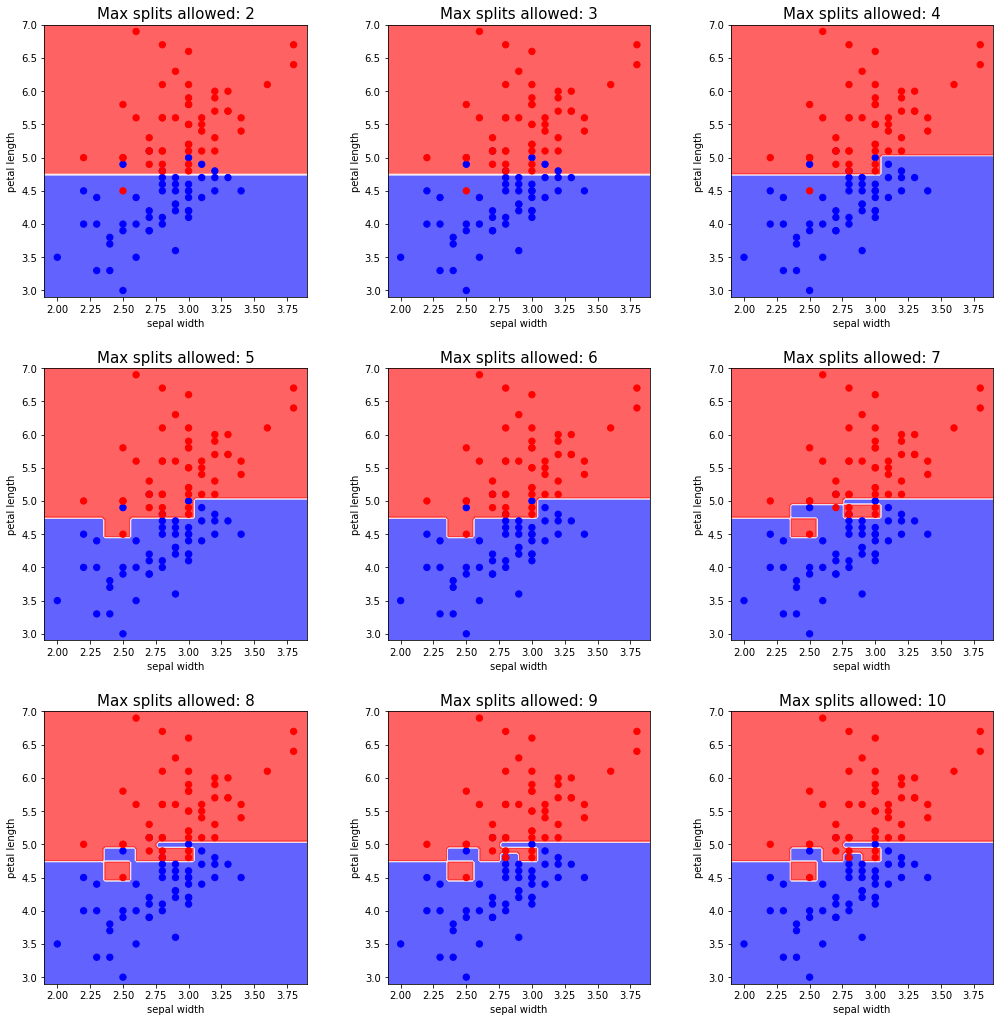
\includegraphics[width=0.8\textwidth]{scatter_plot_illustration.png}

\caption{Illustrating how a researcher visually divides the scatter plot had he or she used only horizontal and vertical lines. This simulation uses a subset of the Iris dataset containing only the Versicolor and Virginica classes, and the Sepal width and Petal length attributes.}
\label{fig:fig1}

\end{figure}

The choice of a tree structure representation was influenced by its common usage in decision making and its ability to display additional information at vertices and arcs, unlike scatter plots that feature only points. The branching structure of the tree also facilitates the analysis of multiple dimensions of the data. \\
Visual features such as colors and gradients aid in emphasizing the data's distribution, while confusion matrices at the tree nodes depict the precise data's density. I named the representation ICC plot, as an acronym of its 3 components: \textbf{I}nduction tree, \textbf{C}onfusion matrices and \textbf{C}olors.

\begin{figure}[H]
\centering
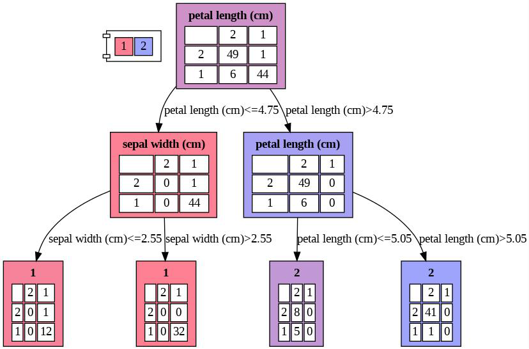
\includegraphics[width=0.6\textwidth]{icc.png}

\caption{ICC with 3 nodes simulate a plain with 3 splits. The data is the same as in \figref{fig1}.}
\label{fig:fig2}

\end{figure}

The ICC plot provides researchers with additional functionality, such as the ability to adjust tree depth to increase or decrease the number of simulated splits of the plane, hide the confusion matrices to focus on data spread, and modify colors. These options are illustrated in \figref{fig3}.

\begin{figure}[H]
        	\centering
           \subfloat{%
              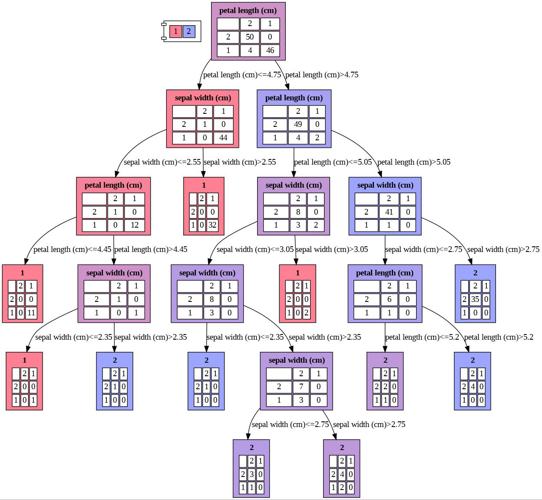
\includegraphics[height=4cm, valign=t]{ICC-v1.png}%
           } 
           \subfloat{%
              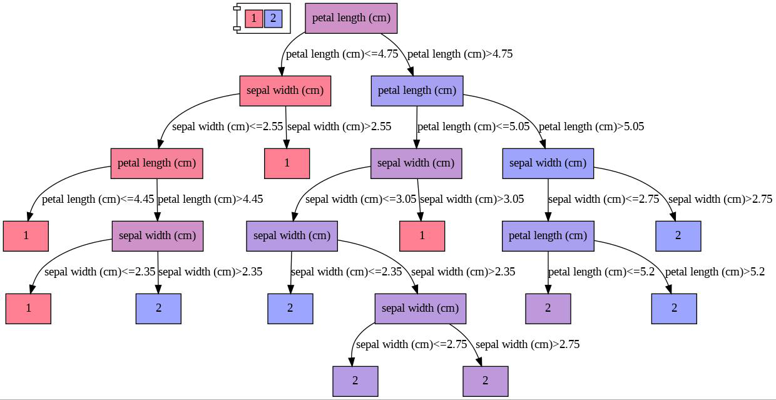
\includegraphics[height=3cm, valign=t]{ICC-v2.png}%
           }
           \subfloat{%
              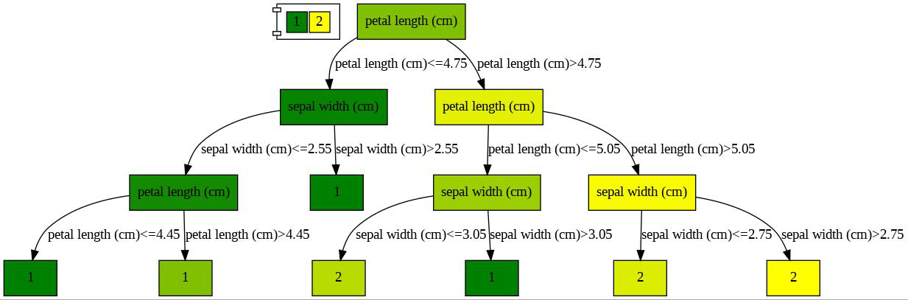
\includegraphics[height=3cm, valign=t]{ICC-v3.png}%
           }
           \caption{Different variations of ICC.}
           \label{fig:fig3}
\end{figure}    

\subsection{The MAGIC tool}
As the ICC plot provides a convenient method to visualize data, it could potentially be utilized to analyze cases where a problem inherent in the data itself (rather than in the training process) results in misclassification. To test this, I propose algorithm \ref{alg:alg1} and provide an API that implements it\footnote{The API not only generates the resulting tree but also enables extracting predicates representing a given test-sample according to it.}. I named the API the MAGIC (\textbf{M}isclassification \textbf{A}nalysis by \textbf{G}raphic \textbf{I}nduction-Tree \textbf{C}lassifier) tool. A sample of the MAGIC algorithm output is presented in \figref{fig3}.
\begin{algorithm}
\caption{MAGIC algorithm}\label{alg:alg1}
\begin{algorithmic}[1]
	\State Build an ICC graph based on the training data.
	\State Trace the path of the test data on the ICC graph:
	\begin{algsubstates}
	\State Update the confusion matrices accordingly at each node.
	
	\State Mark nodes no test-data has passed through at all with white (These represent parts of the space that were present in the training data but are missing in the test data).
	\State Highlight nodes where samples of a different class than the one that appeared in the training set have reached with a double frame. 
\end{algsubstates}
\end{algorithmic}
\end{algorithm}

\begin{figure}[H]
\centering
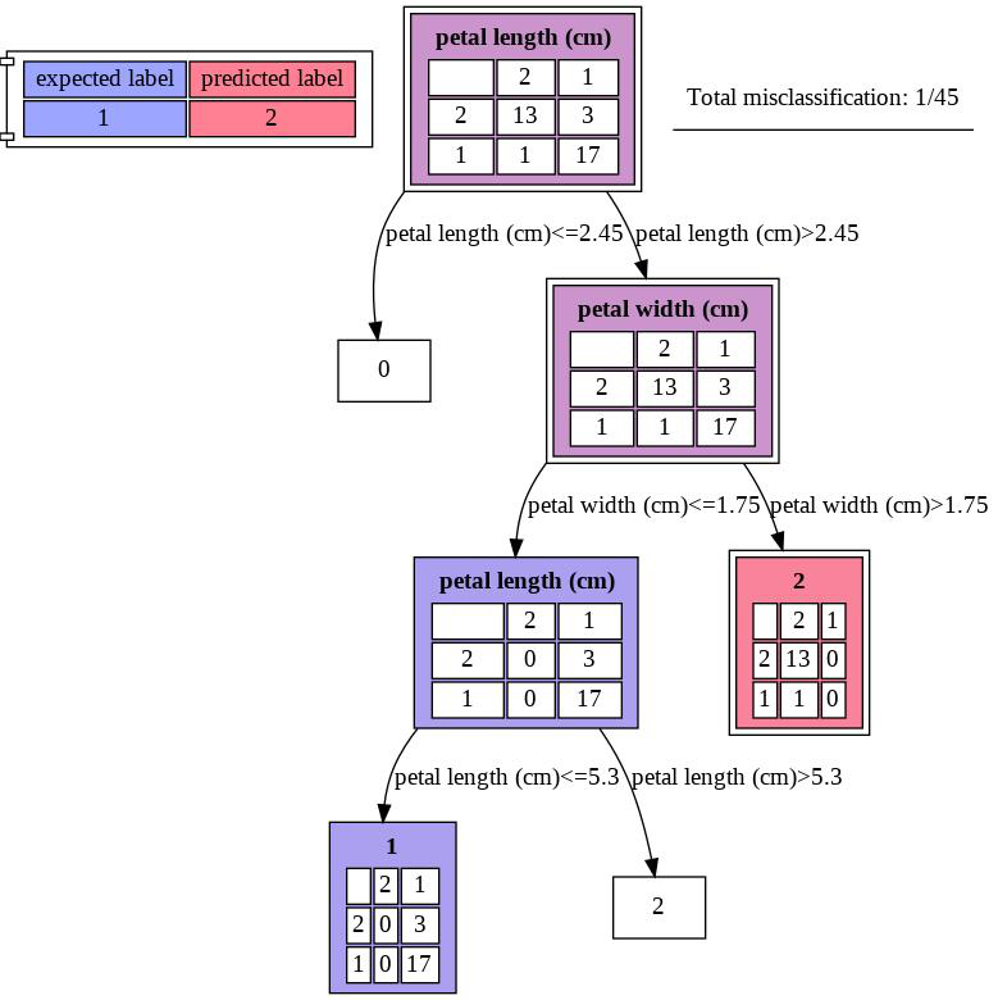
\includegraphics[width=0.5\textwidth]{iris-magic.png}

\caption{Examining test-data of the Iris dataset: The white vertices represent samples that are not present in the test data (for example, irises with a petal length of 2.45 or less). The double-framed vertices reveal that one sample in the test data was misclassified as type 2 when it is actually type 1. This error is understandable as 13 type 2 samples were correctly classified for similar reasons.}
\label{fig:fig3}

\end{figure}

\section{Experimental evaluation}\label{Experimental evaluation}
\subsection{The ICC plot}
I evaluated the performance of the ICC plot by comparing it to Scatter and Jitter plots, as a baseline. To do this, I presented four CS students majoring in Data Science two graphs representing a given dataset: one Scatter (or Jitter) plot, and the other - ICC plot. In the first stage, I asked the students to write down as many observations as possible from each graph. In the second stage, I asked them to determine the relevance of their observations to the classification problem the dataset is used for. Finally, I asked them to share the advantages and disadvantages they came across during this evaluation. I repeated this process with three well-known datasets: Iris, Titanic, and Wisconsin breast cancer data\footnote{Only ten out of the thirty possible attributes in the Wisconsin breast cancer dataset were used in order to simplify the evaluation process.}. The results are in table \ref{table:tab1}.

\begin{table}[h]
\centering
\begin{tabular}{ |m{2cm}|m{6cm}||P{1.7cm}|P{1.7cm}|P{3.5cm}| } 
\hline
\multicolumn{2}{|m{3cm}||}{} & Iris data & Titanic data & Wisconsin breast cancer data \\
\hline
\hline
\multirow{2}{*}{\parbox{4cm}{Scatter\textbackslash\\Jitter plot}} & Mean number of observations according to the graph & 4.25 & 2 & 8.5 \\\cline{2-5}
& Percentage of observations relevant to the classification process &  27.9\% & 50\% & 23.6\% \\
\hline
\multirow{2}{*}{ICC} & Mean number of observations according to the graph & 2 & 2 & 3.5 \\\cline{2-5}
& Percentage of observations relevant to the classification process &  79.1\% & 79.1\% & 75.4\% \\
\hline
\end{tabular}
\caption{Quantity and percentage relevance of insights for each classification problem.}
\label{table:tab1}
\end{table}

The results show that Scatter and Jitter Plots are easier to draw insights from. On average, the scatter plots enabled to generate twice as many insights about the data compared to the ICC plot. However, the percentage of relevant insights for classification is low: for the ICC plot, almost 4/5 of the insights were relevant to the classification process compared to only one third for the Scatter and Jitter plots.\\
The feedback from the subjects indicated that the ICC plot was better suited for analyzing classification problems than Scatter plots, but had two major drawbacks: it was not very intuitive and required them to learn how to use it properly before using it. Additionally, it did not allow for the identification of correlations as can be done with scatter plots.

\subsection{MAGIC Evaluation Process}\label{MAGIC Evaluation Process}
The evaluation of the MAGIC tool was conducted in two stages too. The first stage involved a \textbf{qualitative comparison} of the MAGIC tool's performance with the scatter plot on the three datasets, as well as on a forth additional synthetic dataset demonstrating hidden stratification. The second stage of the evaluation was \textbf{quantitative}: the subjects were presented with the data distribution of the four datasets using both the MAGIC tool and scatter plot. A humorous questionnaire was used to ask them to identify the reason for misclassification based on each of the visualization options.

The qualitative research found that the scatter plot graph is more effective in characterizing global phenomena, such as overlap in the characteristics of samples belonging to different classes, while the MAGIC tool is more useful for analyzing local phenomena, such as samples with identical or almost identical characteristics belonging to different classes. The MAGIC tool was significantly useful for datasets where most of the characteristics were categorical because the scatter plot suffered from overplotting. The MAGIC tool was also found to be more useful in cases where misclassification was due to hidden stratification.
\\The questionnaire results are presented on table \ref{table:tab2}. The subjects reported that the MAGIC tool was reasonably useful for the presented tasks, yet its main disadvantage is the significant learning required to understand its visual complexity.


\begin{table}[h]
\centering
\begin{tabular}{ |m{5cm}||m{5cm}|m{5.5cm}| } 
\hline
Reason for misclassificaion & Number of subjects who correctly identified the phenomenon using a Scatter plot & Number of subjects who correctly identified the phenomenon using the MAGIC tool \\
\hline
\hline
samples with identical characteristics & 0/3 & 2/3 \\
\hline
Samples with overlapping characteristics & 3/3 & 2/3 \\
\hline
Hidden Stratification & 1/3 & 2/3 \\
\hline
\end{tabular}
\caption{Comparison of correct identification of the cause of misclassification using a scatter plot vs. the MAGIC tool.}
\label{table:tab2}
\end{table}

\section{Related work}\label{Related work}
\subsection{Scatter plots limitation}\label{Scatter plots limitation}
Although having quite a few limitations, Scatter plots are widely used. Researchers proposed different improvements to overcome these limitations. I will briefly review a selection of works and solutions.\\
Scatter plots can get cluttered with large datasets and overlapping points, preventing the researcher from correctly assessing the density of the data. This is especially crucial when comparing between different groups. The most famous improvement for that is the Jitter plot, that randomly adjusts point positions. \cite{woodruff1998constant} proposed the VIDA system that plots dots for objects in dense regions and polygonal outlines for objects in sparser regions. \cite{dang2010stacking} suggested addressing the above by arranging points in the third dimension.\\
Another problem is the difficulty of separating overlapping groups in the data. \cite{lee2012ieee} offer to use hierarchical multi-class sampling method to create a simplified, feature-preserving scatter plot visualization. \cite{mayorga2013splatterplots} propose to group dense data points and reveal subgroup relations through the use of contour lines.\\
As plotting in four or more dimensions is impossible, Scatterplot Matrix (SPLOM) is commonly used, yet it imposes new challenges as it doesn’t scale with the features quantity[\citenum{carr1987scatterplot}][\citenum{lehmann2012selecting}].\\
Additional improvements might include employing Scagnostics methods[\citenum{sharma2012determining}], Spatial distortion[\citenum{keim1998gridfit}] and focusing on local patterns[\citenum{shao2016guiding}].

\subsection{Visualizing human decision making processes by trees
}\label{Visualizing human decision making processes by trees}

Trees are broadly used across different disciplines to analyze complex decision making processes. For example, the Ethno-graphic decision tree modeling[\citenum{gladwin1989ethnographic}] is a research method designed to identify the factors that groups of people use in their decision making. In game theory, the decision-making process is formalized using a tree, known as a \textit{game tree}[\citenum{gibbons1997introduction}]. Trees are available to professionals, such as psychological counselors, to aid in the counseling process[\citenum{beck2005ethnographic}] and for service providers to assess service provision[\citenum{harrison2018selecting}]. In political science, decision trees can serve as a tool to analyze election results[\citenum{armengol2020decision}][\citenum{joynersimulating}].

\subsection{Misclassification Analysis}\label{Misclassification Analysis
}
Misclassification analysis is a crucial step in the Data Science pipeline, and as such, development environments designed for data scientists provide a variety of dedicated tools for it. Gestalt-20[\citenum{patel2010gestalt}] enables researchers to compare different samples side by side, making it possible to visually analyze differences between images in entity extraction tasks, or texts in sentiment analysis tasks. ModelTracker[\citenum{amershi2015modeltracker}] is another tool that enables local examination of classification errors.\\
An example of a system in the text domain is EluciDebug[\citenum{kulesza2015principles}], which reports to the user why it classified a certain email in the way it did.\\
Finally, it is important to mention the well-known LIME algorithm[\citenum{ribeiro2016should}], which recommends using simple and interpretable models to investigate the local environment of a misclassified sample.

\section{Conclusion}\label{Conclusion}
In this project I proposed a novel approach to data visualization using tree-structures, which was effective in exploratory data analysis (EDA) and overcame the limitations of scatter plots. While it had limited usefulness in misclassification analysis, it was found to be beneficial in specific cases such as identifying hidden stratification.\\
Throughout this project, I first and foremost learned about the essential steps of the research process. One important takeaways is the significance of thoroughly defining and investigating the research question. In particular, I came across the LIME algorithm at an advanced stage of the project, before it was discussed in class. I was somewhat disheartened to discover a tool that provides some of the functionality of the tools I offer (the MAGIC tool) in a simpler and more convenient manner. On the other hand, it was reassuring to see that the LIME algorithm relies on interpretable models, similar to the tree structure I chose for my own work. It was also encouraging to see that the tools I suggested help in discovering cases like hidden stratification more effectively then LIME. In any case, if I had to name one work that inspired me, it would be the LIME algorithm as it is an elegant, mathematically-supported, and user-friendly tool.\\
Overall, exploring different visualization tools and approaches was a fascinating experience. It provided me with a profound comprehension of the objectives and procedures that researchers undergo when encountering various visualizations.


\setcitestyle{numbers}
\bibliographystyle{plainnat}
\bibliography{bib}

\end{document}